\section{Beispiel Timer}
\begin{minipage}[]{0.49\textwidth}
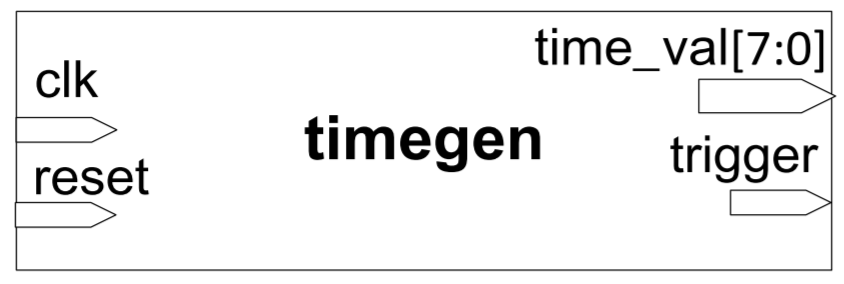
\includegraphics[width = 0.5\textwidth]{pics/timegen.png}

Definition des Bausteins Counter. Die Generic-Variable wird zur Compilezeit definiert.\\
VHDL hat 3 mögliche Zeitpunkte, zu denen ein Parameter definiert werden kann:
\begin{itemize}
\itemsep0em
\item Zur Designzeit - Konstante \texttt{maxcount: integer:= 127};
\item Zur Compilezeit - Generic
\item Zur Laufzeit - Signal
\end{itemize} 
\lstinputlisting[language=VHDL,tabsize=2]{code/genTimer.vhd}

\end{minipage}
\hfill
\begin{minipage}[]{0.49\textwidth}
\lstinputlisting[language=VHDL,tabsize=2]{code/timegen.vhd}
\end{minipage}